\documentclass[
11pt, % Main document font size
a4paper, % Paper type, use 'letterpaper' for US Letter paper
oneside, % One page layout (no page indentation)
twoside, % Two page layout (page indentation for binding and different headers)
headinclude,footinclude, % Extra spacing for the header and footer
BCOR5mm, % Binding correction
]{scrartcl}

\usepackage[
nochapters, % Turn off chapters since this is an article        
beramono, % Use the Bera Mono font for monospaced text (\texttt)
eulermath,% Use the Euler font for mathematics
pdfspacing, % Makes use of pdftex’ letter spacing capabilities via the microtype package
dottedtoc % Dotted lines leading to the page numbers in the table of contents
]{classicthesis} % The layout is based on the Classic Thesis style

\usepackage{arsclassica} % Modifies the Classic Thesis package
\usepackage{minted}
\usepackage{pdfpages}

\usepackage[T1]{fontenc} % Use 8-bit encoding that has 256 glyphs

\usepackage[utf8]{inputenc} % Required for including letters with accents

\usepackage{graphicx} % Required for including images
\graphicspath{{Figures/}} % Set the default folder for images
\usepackage[total={6.5in, 9.0in}]{geometry}

\usepackage{enumitem} % Required for manipulating the whitespace between and within lists

%----------------------------------------------------------------------------------------
%	TITLE AND AUTHOR(S)
%----------------------------------------------------------------------------------------

\title{\normalfont\spacedallcaps{Virtual Watershed Laboratory}} % The article title

\subtitle{\normalfont\spacedallcaps{Plan for 2015: Optimize the Whole}} % The article title

\author{\spacedlowsmallcaps{Matthew A. Turner*}} % The article author(s) - author affiliations need to be specified in the AUTHOR AFFILIATIONS block

%----------------------------------------------------------------------------------------
%	HYPERLINKS
%---------------------------------------------------------------------------------------
\usepackage{hyperref}
\hypersetup{
%draft, % Uncomment to remove all links (useful for printing in black and white)
colorlinks=true, breaklinks=true, bookmarks=true,bookmarksnumbered,
urlcolor=webbrown, linkcolor=RoyalBlue, citecolor=webgreen, % Link colors
pdftitle={Virtual Watershed Laboratory, Plan for 2015: Optimize the Whole}, % PDF title
pdfauthor={\textcopyright}, % PDF Author
pdfsubject={}, % PDF Subject
pdfkeywords={}, % PDF Keywords
pdfcreator={pdfLaTeX}, % PDF Creator
pdfproducer={LaTeX with hyperref and ClassicThesis} % PDF producer
}

\begin{document}
\maketitle % Print the title/author/date block

\setcounter{tocdepth}{2} % Set the depth of the table of contents to show sections and subsections only

\tableofcontents % Print the table of contents
\section*{abstract}

After gathering requirements and working to understand the needs of the 
WC-WAVE waterhsed scientists and modelers, we report the results and present a
proposal for a focusing long-range vision of our final product. We plan to 
reach our goal for this final product by a series of demonstration projects that
in themselves will be publishable works.

In the long run, we plan to build a system that can deliver data through either
a web client or via a Python API. 

{\let\thefootnote\relax\footnotetext{* \textit{Northwest Knowledge Network, 
University of Idaho}}}



\newpage
     

\section{Introduction} % (fold)
\label{sec:intro}

The EPSCoR Tri-State Western Consortium for Water Analysis, Visualization, and Exploration (WC-WAVE)
is made up of a diverse group of researchers from colleges and universities 
throughout the three partner state, Idaho, Nevada, and New Mexico. If nothing else can be said, it's 
sure that large interdisciplinary projects are difficult. However they are proving grounds for 
new ideas and, indeed, new ways of doing science. So today, our job is not just to write software
but to deliver a cyberinfrastructure tool that will enhance the visibility, viability, and 
permanence of the work of watershed scientists and hydrologiests. This tool is the virtual 
watershed and its importance cannot be overstated.

Here are a few paraphrased things I heard at the January meeting:

\begin{itemize}
    \item "So do models run in the Virtual Watershed and if so, how does that work?"
    \item "How can I run HPC-dependent models with the Virtual Watershed?"
    \item (In reference to an IPython demo of the watershed) "Are you sure you wanna show that?"
    \item "I want to be able to arbitrarily use climate forecasts as drivers for my model"
    \item "I want to be able to use inputs gathered for one model in another model"
    \item "Can I track which model is which with the virtual watershed?"
\end{itemize}

With all these competing requests combined with our (CI-Data/Vis) expectations and understanding
of what the watershed scientists expect from the Virtual Watershed, it is no surprise that
there is a lot of confusion around the meaning and purpose of "Virtual Watershed". So let me
propose some definitions that are by no means permanent, but necessary for an intelligible discussion
of how we will make our next round of progress.

\begin{itemize}
    \item \textbf{Virtual Watershed (VW):} a system for intelligently storing 
        \href{http://www.unidata.ucar.edu/software/netcdf/}{netCDF} files and serving
        a variety of output formats. 
    \item \textbf{Adaptors:} Software to facilitate the use of VW-served data. This software may
        be for direct human-VW interaction, VW-model (e.g. using VW-served data as parameters and 
        forcing variables) interaction, or model-to-model, VW-mediated (data-centric) model 
        coupling
    \item \textbf{Virtual Watershed Laboratory (VWL):} The mythical beast that researchers are
        clamoring for. An interactive platform where researchers can search for and download data,
        upload their data to the virtual watershed, and run models that are available for a given
        dataset.
\end{itemize}

To address all these competing demands and confusions, I propose the following way forward:

At a minimum, we provide the web interface that many researchers would like. I propose we
copy David Tarboton's idea for \href{http://www.iemss.org/sites/iemss2014/papers/iemss2014_submission_243.pdf}{HydroShare}, 
which is to have an interface like YouTube but for watershed data. Below is a wireframe idea
that we can target first. I imagine we can make something like this happen in about six months. 
Of course it will take work, but we have some time, and if we focus on making a next-generation
\textit{easy-to-use} framework, we will make a unique contribution to the wellspring of such tools
aimed at enabling earth science activities in general. Here's how I propse we make that happen.

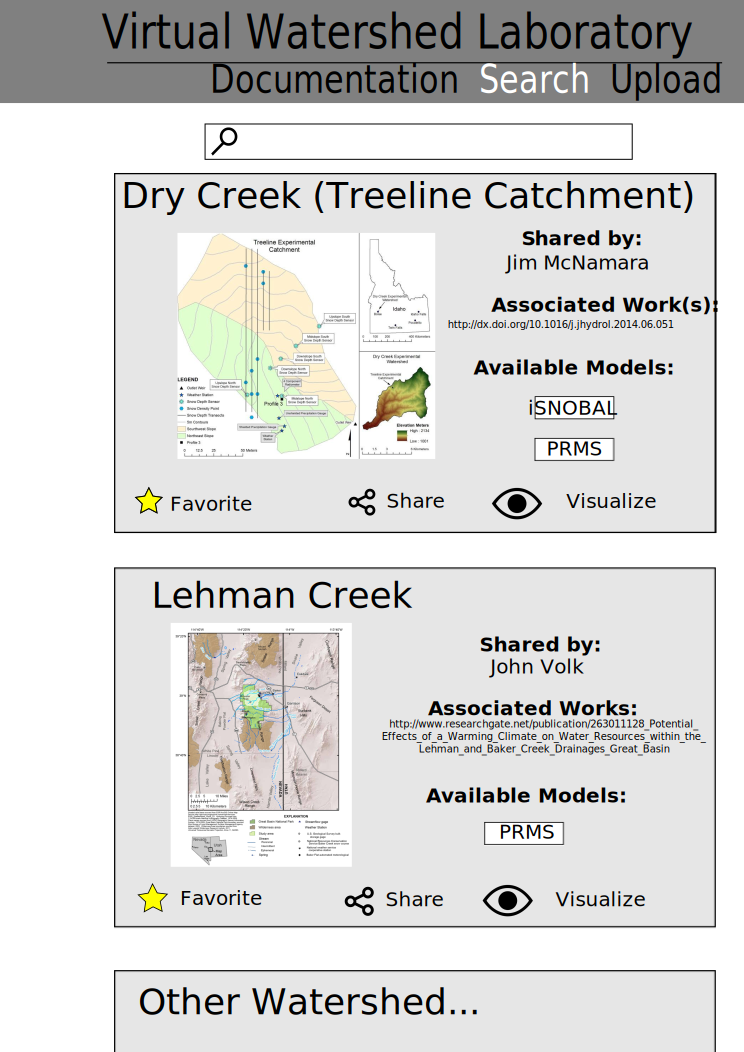
\includepdf{vw_lab_wireframe}

\subsection{Plan and Feature Specifications} % (fold)
\label{sub:Plan}

In that wireframe, there are three separate tasks that need to be done, which can be shared
between UNM, UNR, and UI. As a design principle, I want this interface to be lightweight and to
use a common foundation. Personally, I'm going to use 
\href{http://flask.pocoo.org/docs/0.10/}{Flask}, a Python module for building web apps. There is
also the Pyramid framework that the UNM team is using for the Virtual Watershed, and there's 
also a promising \href{http://www.django-rest-framework.org/}{Django REST framework}. For now,
the particular implementation is not important. If anything, we'd benefit from exploring just what
different frameworks have to offer.

\large{also need to address HPC services}

\subsubsection{University of New Mexico: Virtual Watershed and Submit Web Tool} % (fold)
\label{ssub:UNM_webtool}

At this point in the project, we have put a lot of pressure on the UNM team to make progress
on various fronts to improve the already-impressive virtual watershed. Let me recap the 
development goals for the next quarter here:

\begin{enumerate}
    \item Make netCDF the base format for all VW-hosted data
    \item Expand the functionality such as providing DELETE and returning 
    \item Provide a user interface for submitting new data to the VW
\end{enumerate}

In addition to these, I would add:

\begin{enumerate}
    \item Host production code in the \texttt{master} branch of the \href{https://github.com/tri-state-epscor/virtual-watershed}{virtual-watershed repository}
    \item Include docs on how to install one's own instance of the virtual watershed for local 
        testing and experimentation
    \item Unit tests for the virtual watershed. This is a key element of knowledge creation.
\end{enumerate}

% subsubsection University of Mexico: Virtual Watershed and Submit Web Tool (end)

\subsubsection{University of Nevada: Models as a Service} % (fold)
\label{ssub:UNR_maas}

One very nice feature will be the ability to run models as a web service. This will mean that
on being called, the service will fetch the input data as requested from the VW, save the input
data to the appropriate location on disk, run the model giving updates as it progresses, and 
finally making the output data available for download or visualization via the virtual watershed
laboratory browse page where the model run began.

Using the adaptors, this might be done something like this 
(see \href{http://stackoverflow.com/questions/15182696/multiple-parameters-in-in-flask-approute}{this helpful Stack Overflow answer}):

\begin{minted}{python}
    from flask import Flask

    app = Flask(__name__)

    @app.route("/models/isnobal", methods=['GET'])
    def run_isnobal():
        input_uuid = request.args.get('input_uuid')
        download_urls = vwc.search(model_run_uuid=input_uuid)
        for url in download_urls:
            download_inputs(url)

    @app.route("/models")
    def show_models_doc():
        return MODELS_DOC  # a static documentation string of html and/or js
\end{minted}

% subsubsection University of Nevada: Models as a Service (end)

\subsubsection{University of Idaho: Search interface} % (fold)
\label{ssub:UI_search_interface}

I am in touch with quite a few watershed scientists to continually update our view of what
a useful product is for them. Because of this, I've decided to take on the lead for 
producing the browsing page that I've included in the wire frame. I plan on doing some 
shape-shifting as I've had requests to provide new infrastructure for modellers, and I have 
more hands-on knowledge of running the models. That's why I think we'll have a UI/UNR 
direct collaboration that will have weekly team meetings to check in on progress.

% subsection Plan name (end)

\section{Design Philosophy} % (fold)
\label{sec:design_philosophies}
The design plans above are guided by some design philosophies which are wisely reviewed in 
Mary and Tom Poppendieck's \textit{Implementing Lean Software Development}. The "seven
principles of lean software development" are:

\begin{enumerate}
    \item Eliminate Waste
        \begin{itemize}
            \item Difficult for us, because a year in our goals and requirements still aren't clear
        \end{itemize}
    \item Build Quality In
        \begin{itemize}
            \item Do this with unittests and get users using our platform ASAP
        \end{itemize}
    \item Create Knowledge
        \begin{itemize}
            \item Arguably our main "product" here is the addition of what we (CI-Data/Vis) have 
                learned in building the software backbone of this interdisciplinary project
            \item This requires publicly available software with reliable documentation
            \item We need detailed plans and weekly reports within our teams
        \end{itemize}
    \item Defer Commitment
        \begin{itemize}
            \item Myth: planning is commitment. D.D. Eisenhower: "In war plans are useless but 
                planning is indispensible"
            \item By deferring commitment to specific models or model interactions, we free 
                ourselves to deliver incremental products fast
        \end{itemize}
    \item Deliver Fast
        \begin{itemize}
            \item By delivering fast we initiate a more rapid user feedback/product improvement loop
        \end{itemize}
    \item Respect People
        \begin{itemize}
            \item Hopefully we can all fill our roles as well as ask for help or raise flags when
                some part is too much. Anyone can "stop the line".
        \end{itemize}
    \item Optimize the Whole
        \begin{itemize}
            \item By focusing on the wireframe and a larger-scale plan, we avoid prematurely
                optimizing a subunit of the VWL
        \end{itemize}
\end{enumerate}
% section design_philosophies (end)

\section{Science Situation} % (fold)
\label{sec:science}

\subsection{tl;dr} % (fold)
\label{sub:tl;dr}

At this point, I propose we delay committing to specific scientific applications beyond
running models for which we have fully-built inputs. If we do this well, extending our
functionality to some more interactive modifications, and even the mega-bonus goal of
arbitrary model coupling, will fit in naturally to the architecture we build today.


% subsection tl;dr (end)

\subsection{Justification and details} % (fold)
\label{sub:Justification and details}

% subsection Justification and details (end)

As I've already said, our customers are the watershed scientists and modelers. Our product
should serve them. I think at a minimum, the web app that I've described above, though 
simple, would serve a purpose. It would allow researchers to publish their data and models,
allow others to run the model and interactively visualize the results, and with some 
modification, allow researchers or students to tweak parameters. However, if all we have
is a YouTube for watershed science, then some of the loftier goals that have been discussed,
for example arbitrarily coupling of climate and hydrological models, is not really possible.

In conversations with researchers doing things that sounded possible are actually not. 
I thought that it'd be possible to arbitrarily run an iSNOBAL model on some data that
was in a general format in the watershed, but originally curated for use in some other model.
This is not possible. Modellers speak of "building" specific, e.g. iSNOBAL or PRMS, models.
What this means is generating parameters that act as constants for the entire model run. 
An example parameter found in both PRMS and iSNOBAL is albedo, or the \href{https://www.esr.org/outreach/glossary/albedo.html}{fraction of solar energy (in the short wave) reflected back into space from Earth}. 
This constant is not the same for every watershed. It must not only be approximated,
but calibrated with human interaction. It may be automatable, but that is a difficult 
problem that we should consider outside of the scope of this project.

So then what is within the scope of our project? That is still an open question, but
according to John Volk, once a model is "built" it may be possible to modify certain 
inputs, like temperature. Research would be needed on the details of each model for
the proper way to do this, but this would at least serve an educational purpose. New students
of hydrology and modeling could interactively play with these hosted models and model 
forcings. One modeller in the PRMS/Watershed Hydrology Giants group thought that 
an interactive map with the ability to change the vegetation type (a code from 0 - 4 for the
increasing extent of cover). 

% section science (end)
\end{document}
